\section{Giới thiệu}

\subsection{Giới thiệu về Question Answering}
Lĩnh vực \emph{Truy hồi thông tin (Information Retrieval)} là một lĩnh vực tập trung vào tìm kiếm tài liệu có bản chất \emph{phi cấu trúc (unstructured)} như văn bản, hình ảnh, video\dots sao cho \emph{phù hợp (relevant)} với một \emph{nhu cầu thông tin (information need)} nào đó, từ một \emph{tập hợp dữ liệu lớn (large collections)}.\\

Trong lĩnh vực đó, nhiệm vụ \emph{hỏi đáp (Question Answering – QA)} là nhiệm vụ tự động trả lời những câu hỏi được đưa ra dưới dạng ngôn ngữ tự nhiên. Các câu hỏi trong một miền ứng dụng cụ thể có thể được trả lời thông qua các kỹ thuật xử lý ngôn ngữ tự nhiên. Theo đó, một hệ thống Question Answering sẽ tìm ra câu trả lời cho một câu hỏi bằng cách truy vấn hoặc tìm kiếm ở trong một hệ tri thức nào đó, có thể là một nguồn thông tin, hay một kho kiến thức\dots. Thông thường, hệ tri thức đó sẽ được cung cấp cho hệ thống từ một vài thông tin trước đó, một vài tài liệu có sẵn, hay từ một trang web chứa một lượng thông tin rất đầy đủ như \href{https://www.wikipedia.org}{Wikipedia}.\\

Tuỳ thuộc vào lượng thông tin có sẵn để hỗ trợ trong việc đưa ra câu trả lời, hệ thống Question Answering có thể được chia thành hai loại, bao gồm:
\begin{itemize}
    \item \textbf{Closed-domain Question Answering:} trả lời những câu hỏi liên quan đến một miền ứng dụng nhất định, chẳng hạn như trong lĩnh vực Y tế, hoặc lĩnh vực Chính trị\dots
    \item \textbf{Open-domain Question Answering:} trả lời những câu hỏi liên quan đến mọi thứ có thể, và cần phải dựa vào một kho kiến thức đủ rộng lớn. Một ví dụ của loại hệ thống này là \href{https://arxiv.org/abs/1704.00051}{DrQA}, được phát triển bởi \href{https://research.fb.com}{Facebook Research}. Theo đó, nguồn dữ liệu được cung cấp cho hệ thống DrQA là một lượng lớn các bài viết trên Wikipedia, và do những bài viết đó liên quan đến rất nhiều chủ đề khác nhau, nên hệ thống này có thể được coi là một hệ thống Open-domain Question Answering.
\end{itemize}

\subsection{Các tập dữ liệu nổi tiếng}
Đối với nhiệm vụ Question Answering, để có thể hỗ trợ trong việc huấn luyện và đánh giá một hệ thống, cộng đồng Xử lý ngôn ngữ tự nhiên đã tạo ra một số tập dữ liệu đã được chuẩn hoá. Trong các tập dữ liệu, dữ liệu của mỗi câu hỏi thường bao gồm ba thành phần cơ bản như sau:

\begin{itemize}
    \item \lstinline{"question"}: là một câu hỏi để huấn luyện hoặc đánh giá.
    \item \lstinline{"text"}: là một đoạn văn có thể chứa câu trả lời cho câu hỏi, hoặc không chứa bất kỳ câu trả lời nào.
    \item \lstinline{"answer"}: là câu trả lời cho câu hỏi, có thể có hoặc không tuỳ vào tập dữ liệu huấn luyện hay đánh giá.
\end{itemize}

Trong số các tập dữ liệu đó, có một số tập dữ liệu được sử dụng phổ biến như sau, chủ yếu phù hợp với hệ thống Open-domain Question Answering:

\begin{enumerate}
    \item \textbf{\href{https://rajpurkar.github.io/SQuAD-explorer/}{Stanford Question Answering Dataset (SQuAD)}:} là một bộ dữ liệu được tạo ra bởi các nhà nghiên cứu tại Đại học Stanford. Bộ dữ liệu này bao gồm hơn 100,000 câu hỏi liên quan đến một số chủ đề có trên Wikipedia, với câu trả lời cho mỗi câu hỏi là một hoặc một vài cụm từ có trong đoạn văn tương ứng với chủ đề trên Wikipedia. Tuy nhiên, trong một vài dữ liệu, câu hỏi có thể không có câu trả lời.
    
    \item \textbf{\href{https://ai.google.com/research/NaturalQuestions}{Natural Questions (NQ)}:} là một bộ dữ liệu được cung cấp bởi Google. Bộ dữ liệu này bao gồm hơn 300,000 câu hỏi được người dùng hỏi trong thực tế qua công cụ Google Search, với câu trả lời được trích xuất trong một đoạn của một bài viết tại Wikipedia.
    
    \item \textbf{\href{https://quac.ai/}{Question Answering in Context (QuAC)}:} là một bộ dữ liệu liên quan đến hành động tìm kiếm thông tin trong một cuộc hội thoại giữa một học sinh và một giáo viên. Trong bộ dữ liệu này, học sinh sẽ đưa ra một loạt các câu hỏi về một chủ đề trên Wikipedia, và câu trả lời sẽ được giáo viên đưa ra thông qua những đoạn ngắn của bài viết đó trên Wikipedia. Bộ dữ liệu này bao gồm khoảng 100,000 cặp câu hỏi - câu trả lời.
    
    \item \textbf{\href{https://github.com/facebookresearch/ELI5}{ELI5 (Explain Like I’m Five)}:} là một bộ dữ liệu được tạo ra bởi Facebook Research, bao gồm hơn 270,000 cặp câu hỏi - câu trả lời từ \href{https://www.reddit.com/r/explainlikeimfive/}{subreddit ELI5}, cùng với một số dữ liệu trên CommonCrawl.
    
    \item \textbf{\href{https://arxiv.org/pdf/1611.09830.pdf}{NewsQA}:} là một tập dữ liệu bao gồm hơn 100,000 cặp câu hỏi - câu trả lời liên quan đến các chủ đề trên trang báo điện tử \href{https://www.cnn.com}{CNN}.
\end{enumerate}

\subsection{Kiến trúc của một hệ thống Open-domain Question Answering}
Trong một bài báo được đưa ra bởi \href{https://arxiv.org/abs/2008.02637}{Lewis, et al., 2020}, kiến trúc của hệ thống Open-domain Question Answering có thể được phân thành 3 loại, theo mức độ phức tạp tăng dần như sau:

\begin{itemize}
    \item \textbf{Retriever - Reader:} một hệ thống có thể nhớ và đưa ra câu trả lời cho một câu hỏi đã được huấn luyện từ trước.
    \item \textbf{Retriever - Generator:} một hệ thống có thể trả lời những câu hỏi chưa được biết trước, bằng cách chọn ra câu trả lời phù hợp nhất trong quá trình huấn luyện.
    \item \textbf{Generator:} một hệ thống có thể trả lời những câu hỏi chưa được biết trước, trong đó, câu trả lời của câu hỏi đó không có trong quá trình huấn luyện.
\end{itemize}

3 loại kiến trúc được mô tả như ở Hình \ref{fig:archs} dưới đây.
\begin{figure}[h!]
    \centering
    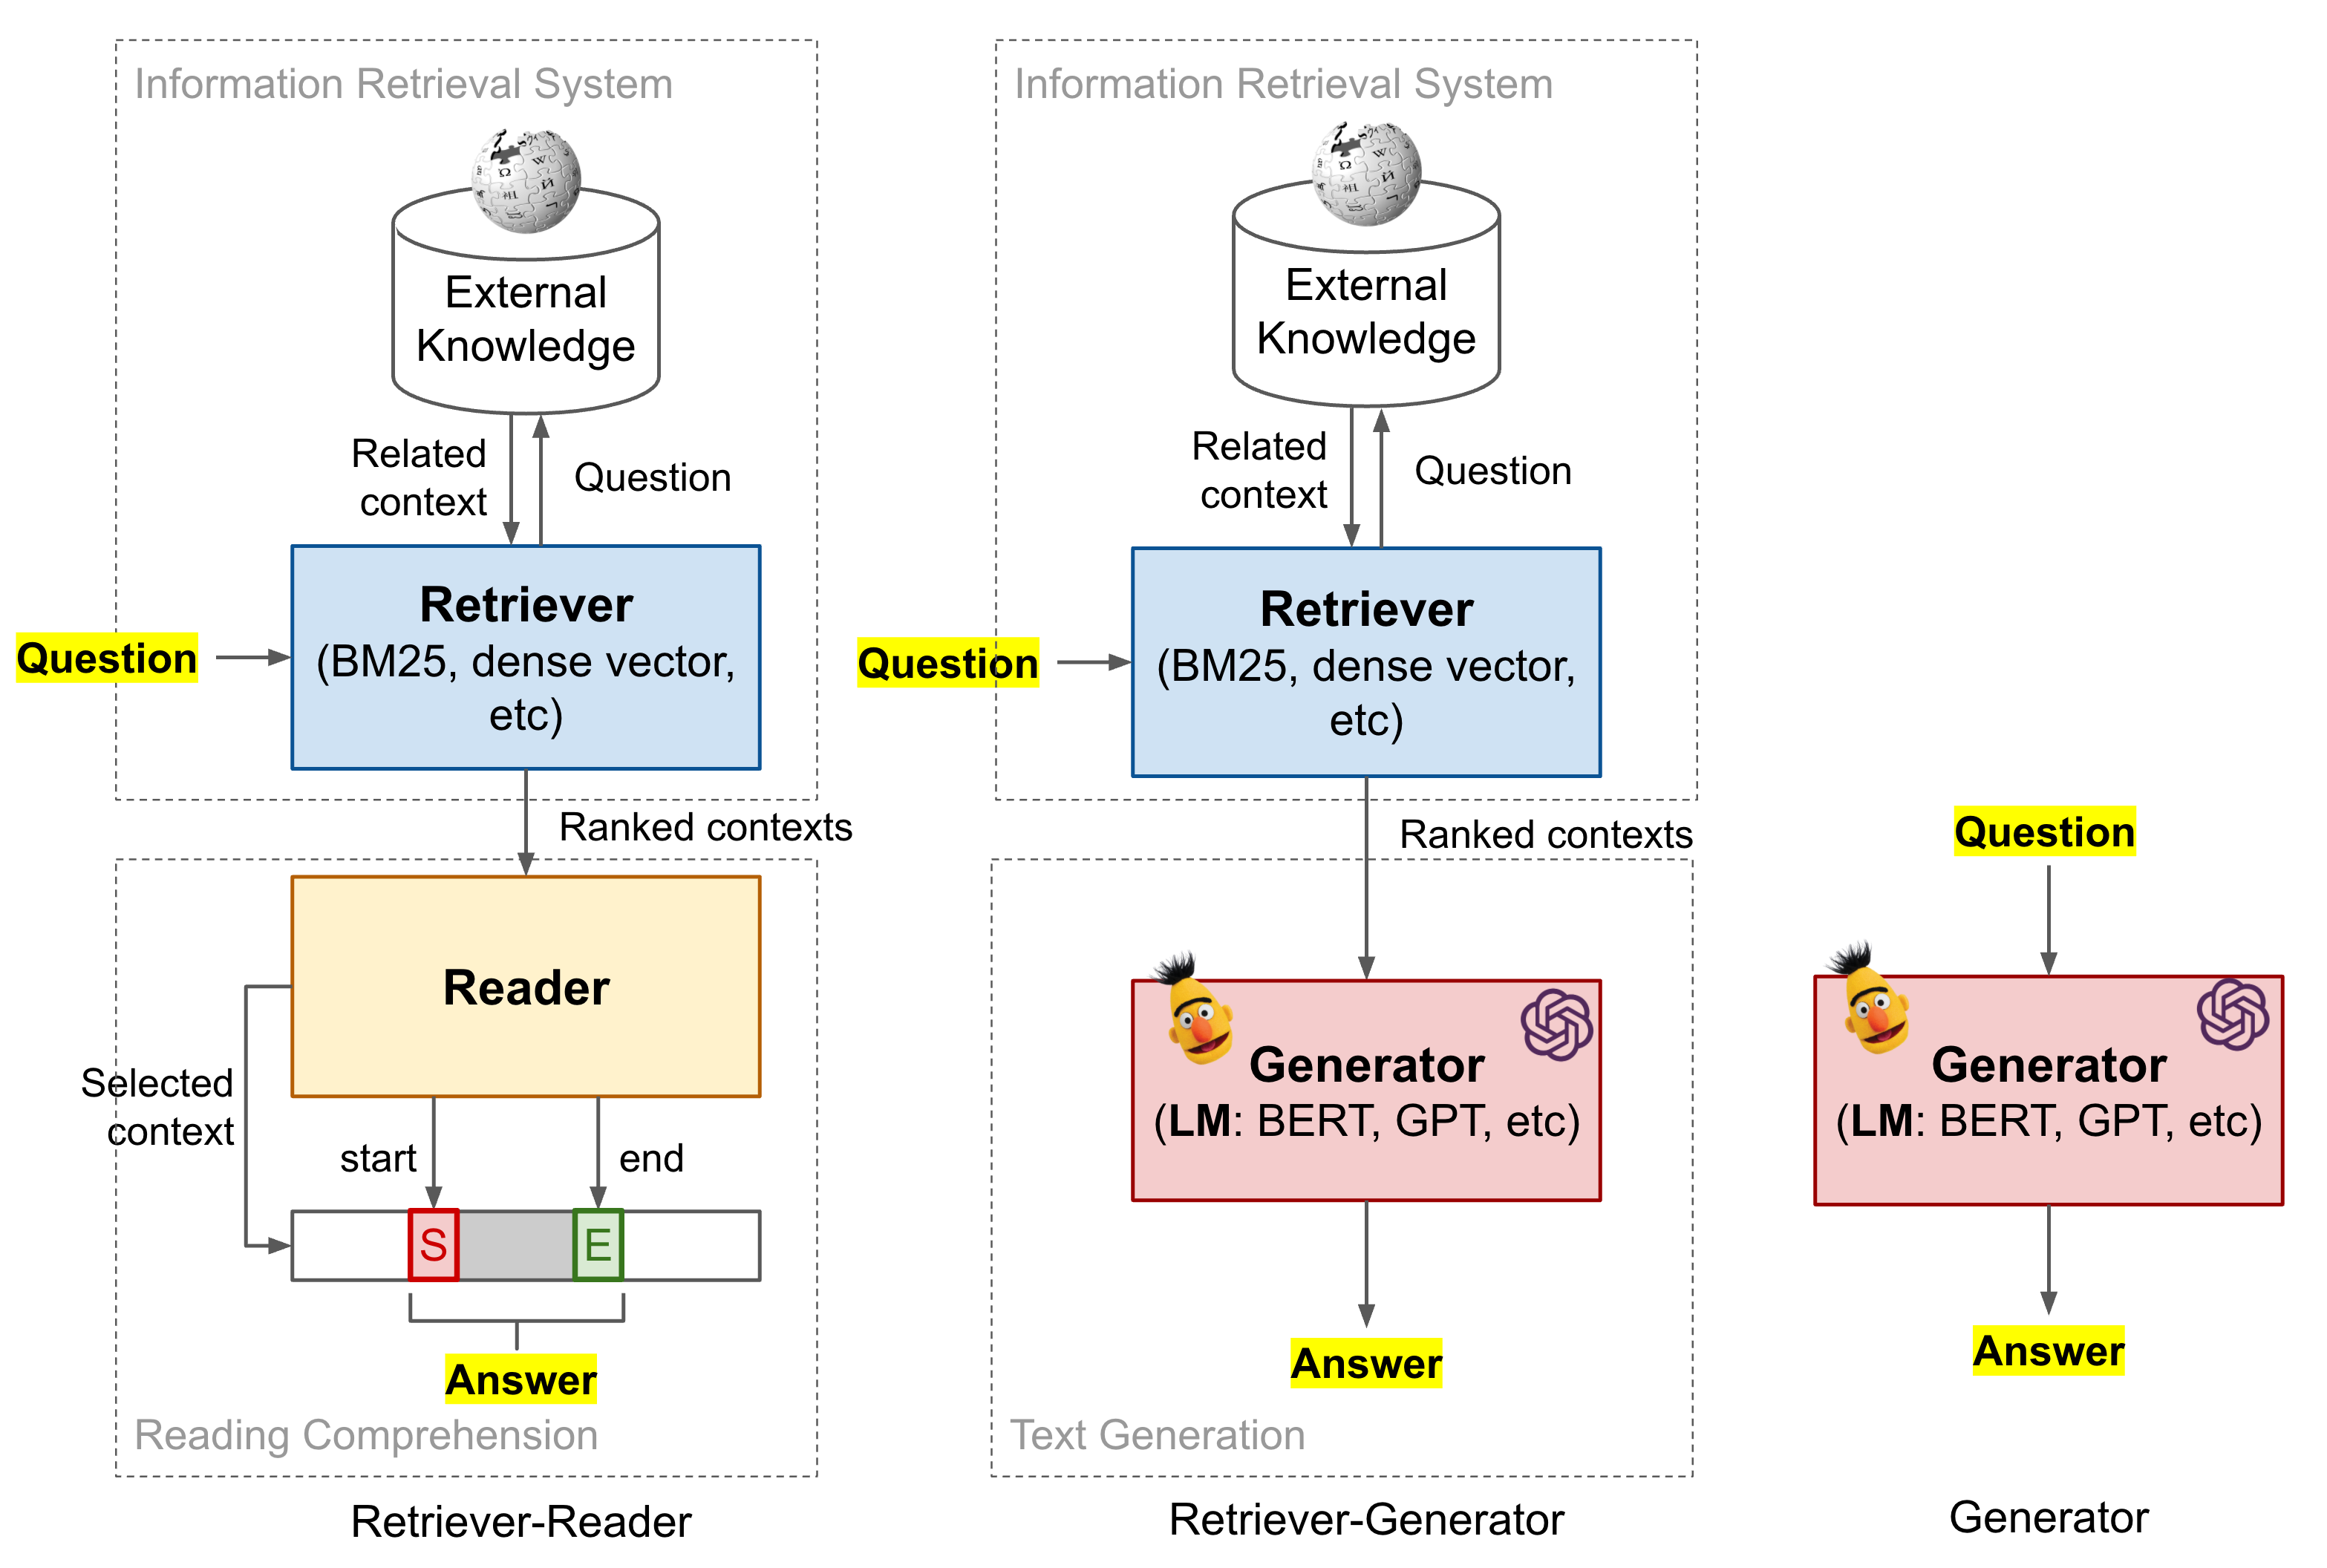
\includegraphics[width=\linewidth]{img/arch/archs.png}
    \caption{Tổng quan về ba kiến trúc của hệ thống Open-domain Question Answering}
    \label{fig:archs}
\end{figure}

\subsubsection{Kiến trúc Retriever - Reader}
Đối với kiến trúc này, khi cần trả lời một câu hỏi, nếu một hệ thống không có bất kỳ thông tin nào, hoặc không đủ lớn để có thể ghi nhớ thông tin có trong tập dữ liệu huấn luyện, hệ thống đó sẽ khó có thể đưa ra một câu trả lời chính xác cho câu hỏi đó. Chính vì vậy, với kiến trúc này, hệ thống cần phải được cung cấp một kho kiến thức rộng lớn, chẳng hạn như Wikipedia, để từ đó có thể xác định được những đoạn có thể liên quan đến câu trả lời.\\

Theo đó, quá trình tìm kiếm câu trả lời cho một câu hỏi nào đó có thể được chia ra thành 2 bước như sau:
\begin{enumerate}
    \item Xác định được đoạn có thông tin liên quan đến câu hỏi trong kho kiến thức được cung cấp,
    \item Trích xuất được câu trả lời trong đoạn thông tin nhận được.
\end{enumerate}

\begin{figure}[h!]
    \centering
    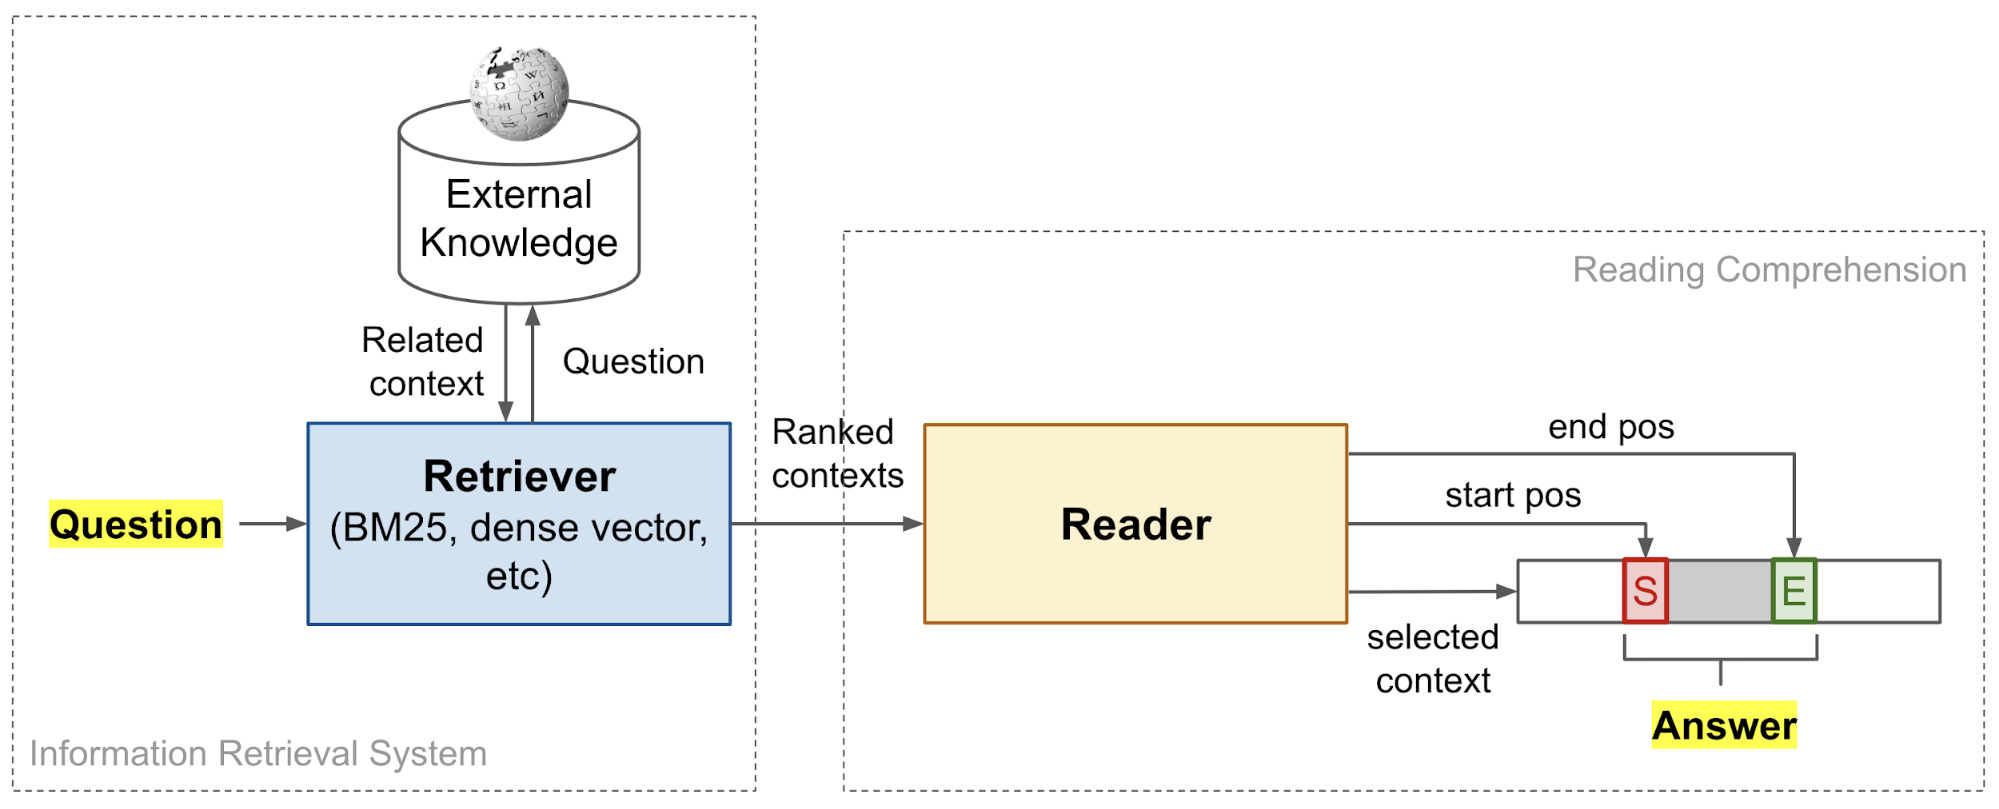
\includegraphics[width=\linewidth]{img/arch/QA-retriever-reader.png}
    \caption{Kiến trúc Retriever - Reader}
    \label{fig:arch_rr}
\end{figure}

Kiến trúc này được đưa ra lần đầu tiên tại bài báo \qq{Document retriever Question-Answering} bởi \href{https://arxiv.org/abs/1704.00051}{Chen et al., 2017}. Theo đó, 2 thành phần Retriever và Reader có thể được huấn luyện và cài đặt một cách độc lập, hoặc được huấn luyện cùng nhau.

\subsubsubsection{Thành phần Retriever}
Để tạo ra thành phần Retriever, có 2 cách tiếp cận phổ biến là sử dụng một hệ thống truy hồi thông tin dựa vào các đặc trưng sau khi áp dụng TF-IDF (cách truyền thống), hoặc dựa vào các embedding vectors của đoạn văn được tạo bởi mạng nơ-ron (cách hiện đại).\\

\begin{flushleft}
\textbf{Cách truyền thống}\\
\end{flushleft}

Mô hình \textbf{DrQA} sử dụng một cách tìm kiếm hiệu quả dựa vào mô hình vector space. Theo đó, mỗi truy vấn và mỗi đoạn văn được biểu diễn theo một vector bag-of-word, trong đó mỗi từ được biểu diễn bởi một trọng số tính theo phương pháp TF-IDF (term frequency $\times$ inverse document frequency). Chi tiết về mô hình này sẽ được mô tả tại \textbf{Mục 2}.\\

\begin{flushleft}
\textbf{Cách hiện đại sử dụng mạng nơ-ron}\\
\end{flushleft}

Thay vì biểu diễn đoạn văn theo một vector space thưa, với các phương pháp tiên tiến như mạng nơ-ron (chẳng hạn như MLP, LSTM, bidirectional LSTM\dots), một đoạn văn có thể được biểu diễn dưới dạng một dense vector. Theo đó, một số mô hình đi theo cách tiếp cận sau:
\[
    h_x = E_x(x) \qquad h_z = E_z(z) \qquad score(x, z) = h_x^Th_z
\]

\begin{enumerate}
    \item Trích xuất dense vector biểu diễn câu hỏi $x$ và đoạn văn $z$ bằng cách sử dụng một mạng nơ-ron,
    \item Nhân 2 vector với nhau để thu được điểm đánh giá tương quan, từ đó xếp hạng những đoạn văn có mức độ liên quan đến câu hỏi cao nhất.
\end{enumerate}

\subsubsubsection{Thành phần Reader}
Thành phần Reader được sử dụng với mục đích trích xuất được câu trả lời từ một đoạn văn nhất định. Theo đó, có một số phương pháp sử dụng mô hình mạng nơ-ron được áp dụng phổ biến đối với bài toán này, bao gồm:
\begin{itemize}
    \item \textbf{Bi-directional LSTM:} là mô hình được sử dụng trong DrQA.
    \item \textbf{Các mô hình BERT}
\end{itemize}

\begin{figure}[h!]
    \centering
    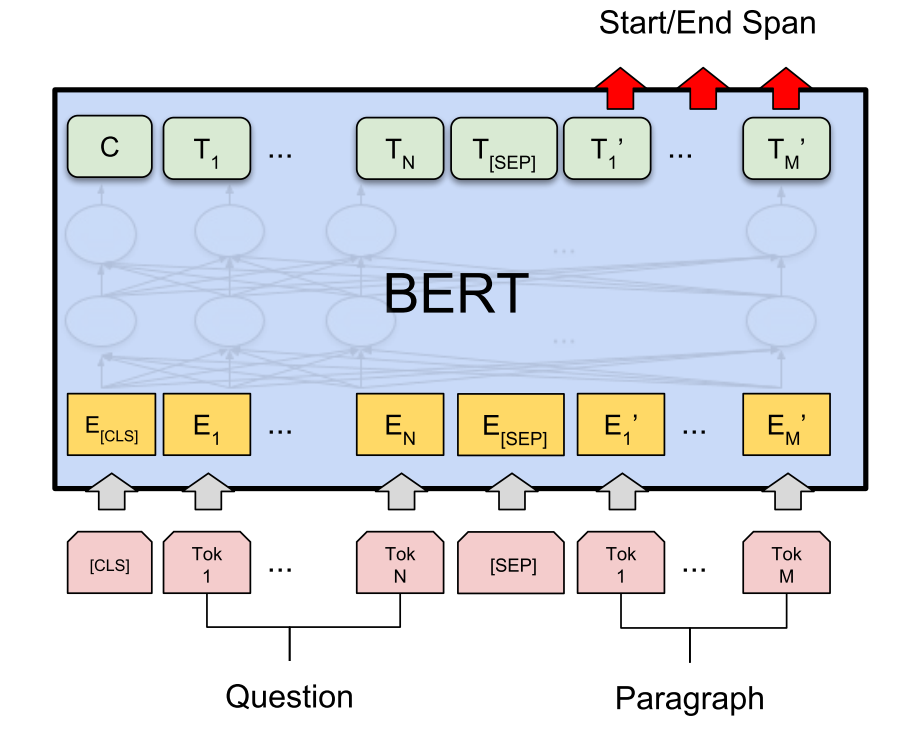
\includegraphics[width=0.5\linewidth]{img/arch/BERT-RC.png}
    \caption{Mô hình BERT được sử dụng trong hệ thống Question Answering}
    \label{fig:arch_rr_bert}
\end{figure}


\subsubsection{Kiến trúc Retriever - Generator}
Khác với kiến trúc Retriever - Reader, đối với kiến trúc Retriever - Generator, mục tiêu của bước thứ 2 là sinh ra một câu trả lời cho câu hỏi hơn là trích xuất câu trả lời dựa vào một đoạn văn.

\begin{figure}[h!]
    \centering
    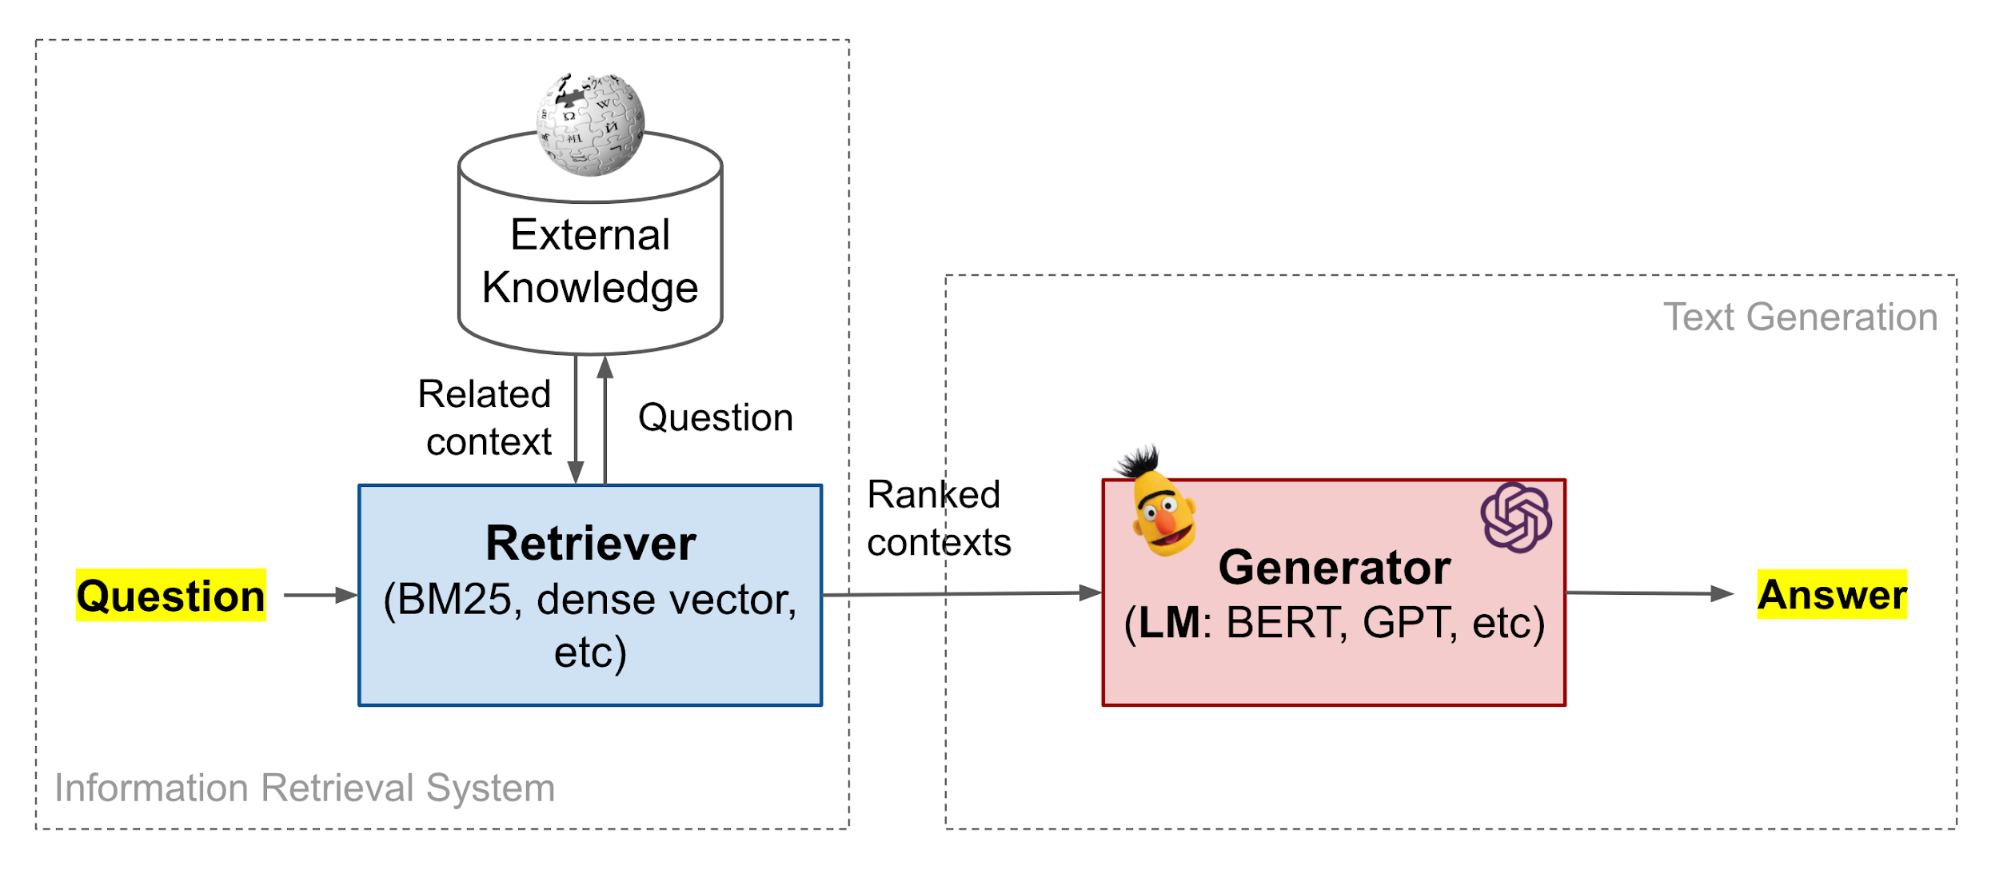
\includegraphics[width=\linewidth]{img/arch/QA-retiever-generator.png}
    \caption{Kiến trúc Retriever - Generator}
    \label{fig:arch_rg}
\end{figure}

Theo đó, sau khi những đoạn văn đã được tìm kiếm và xếp hạng, thành phần Generator sẽ sử dụng mô hình BERT, GPT hoặc các mô hình tương tự để có thể sinh ra câu trả lời cho câu hỏi một cách hiệu quả nhất. Một mô hình hệ thống đặc trưng cho kiến trúc này là \emph{RAG} (Retrieval-Augmented Generation), được giới thiệu bởi \href{https://arxiv.org/abs/2005.11401}{Lewis et al., 2020}.

\begin{figure}[h!]
    \centering
    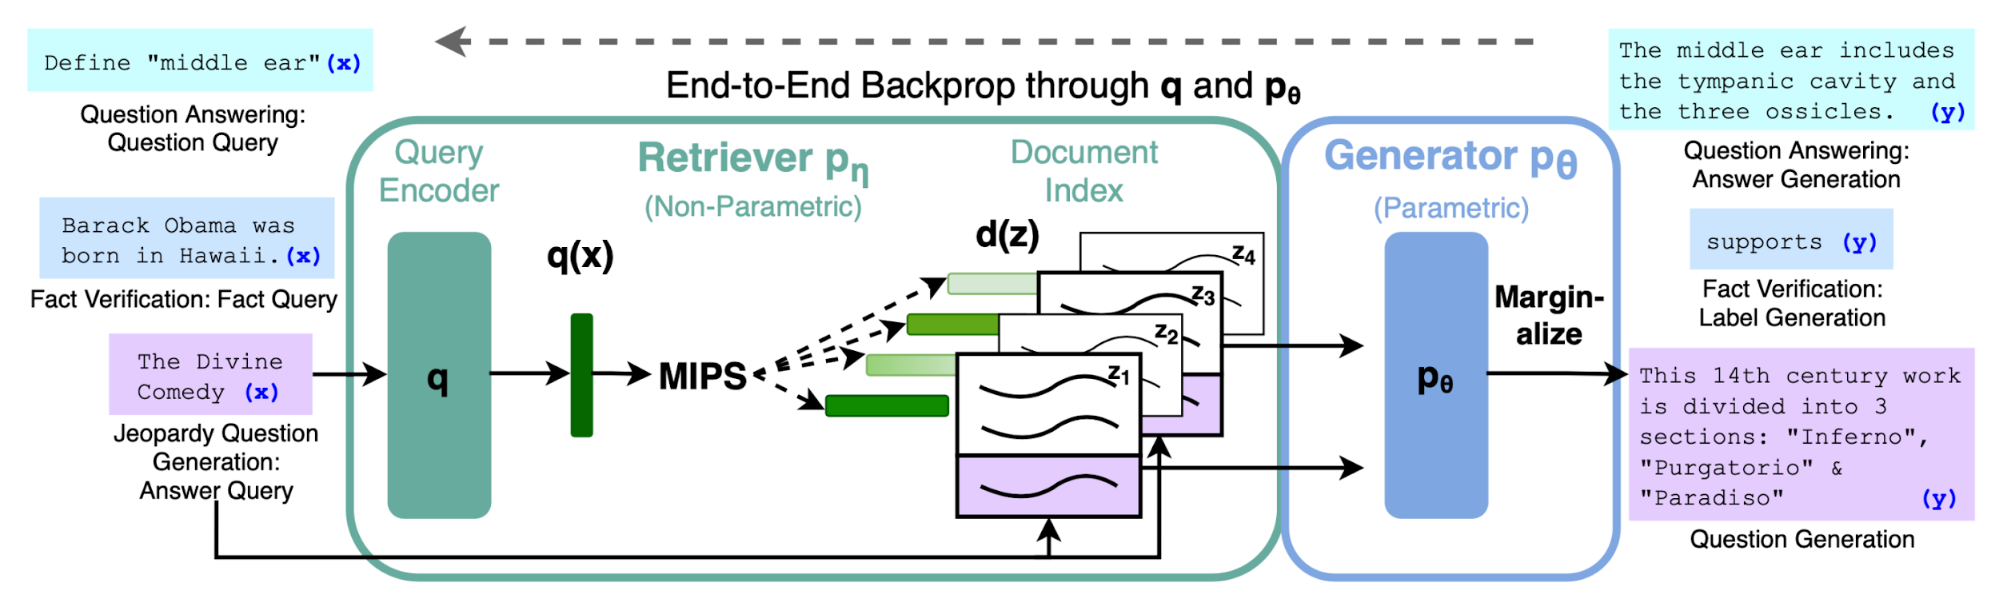
\includegraphics[width=\linewidth]{img/arch/RAG.png}
    \caption{Mô hình RAG}
    \label{fig:arch_rg_rag}
\end{figure}

\subsubsection{Kiến trúc Generator}
Đối với một số mô hình ngôn ngữ có kích cỡ lớn, chúng đã được huấn luyện dựa trên một tập lớn các dữ liệu văn bản, từ đó chúng có thể ghi nhớ những kiến thức thông qua các trọng số trong những mô hình đó. Chính vì vậy, những mô hình đó có thể được sử dụng để trả lời những câu hỏi mà không cần cung cấp một ngữ cảnh cụ thể.

\begin{figure}[h!]
    \centering
    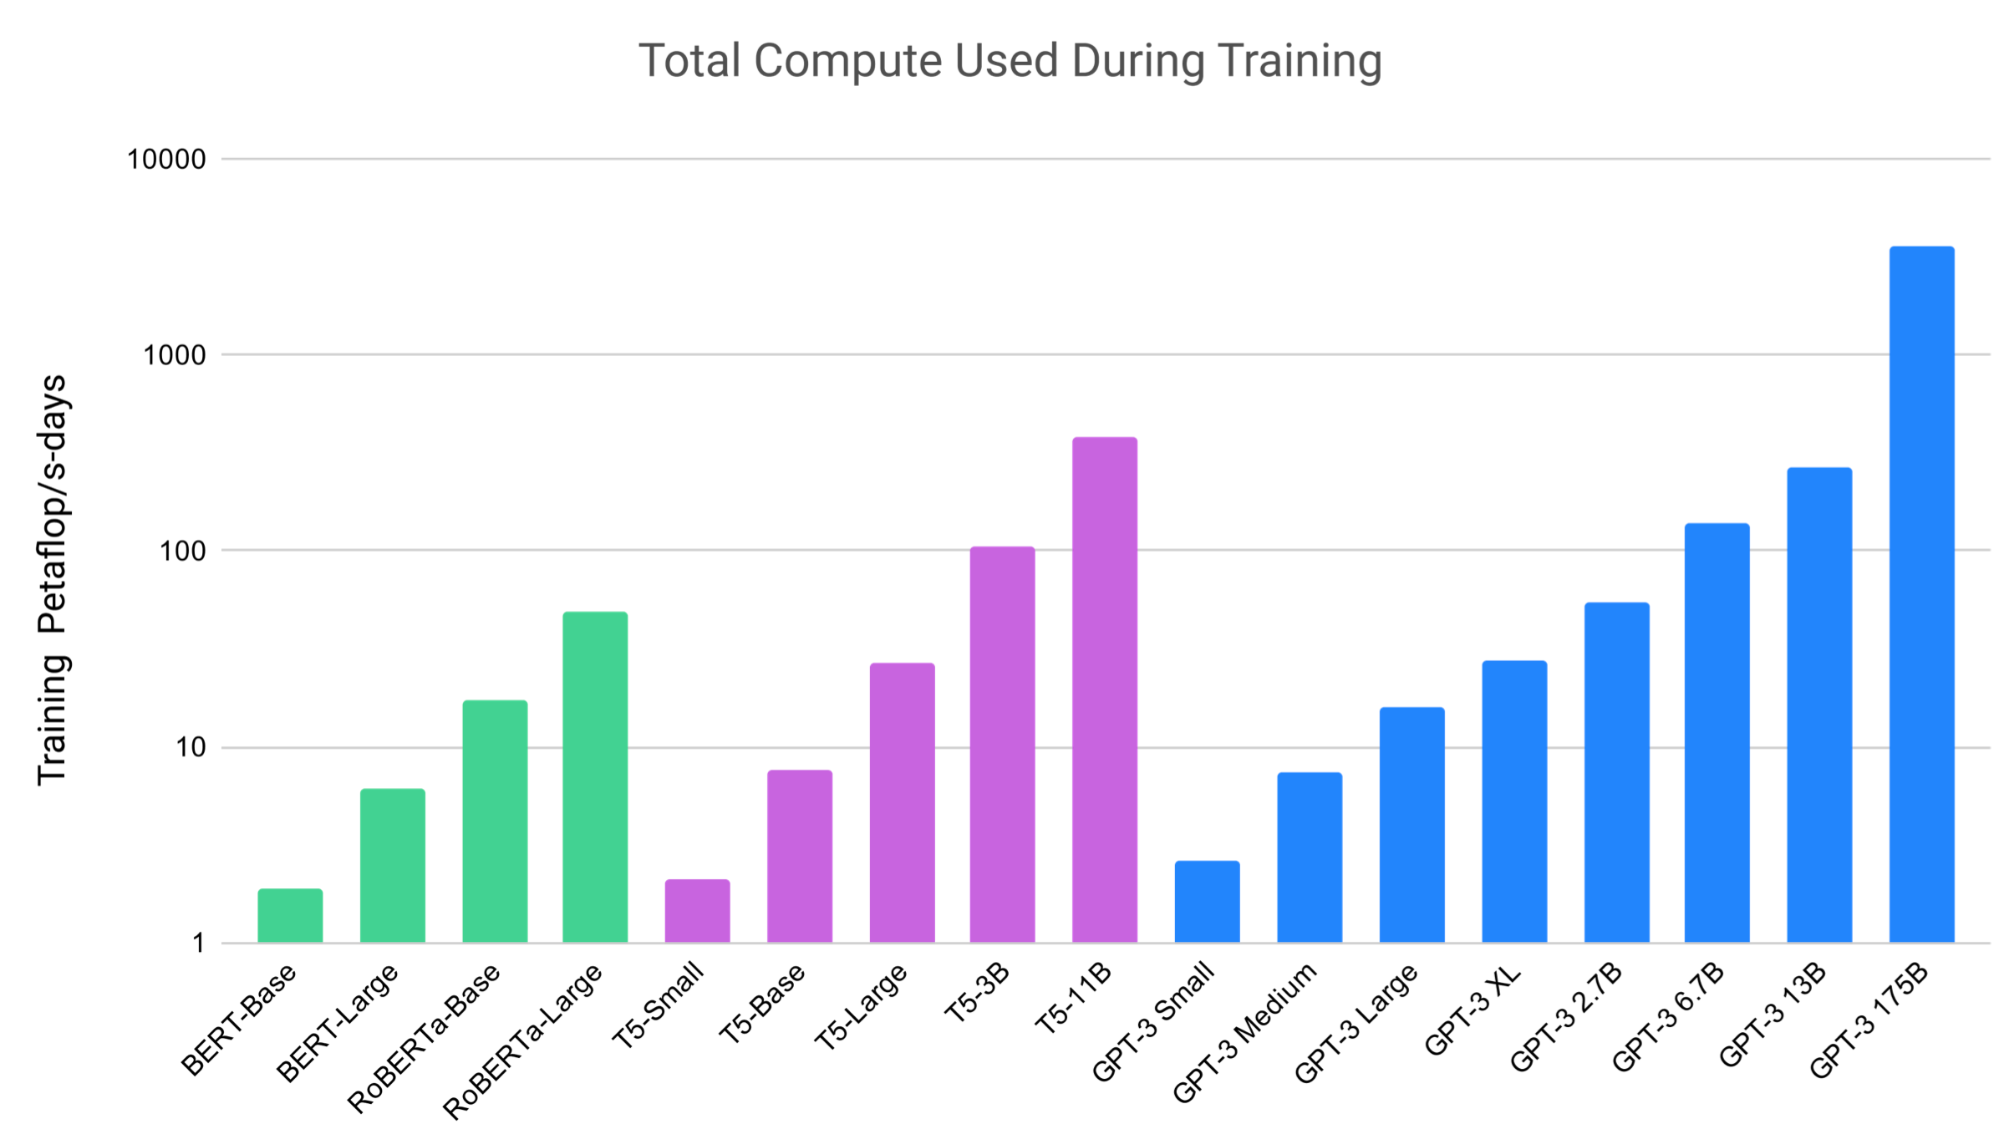
\includegraphics[width=\linewidth]{img/arch/LM-compute.png}
    \caption{Kích cỡ của một số mô hình ngôn ngữ phổ biến}
    \label{fig:arch_lm}
\end{figure}

Theo đó, trong một bài báo được giới thiệu bởi \href{https://arxiv.org/abs/2002.08910}{Roberts et al. (2020)}, họ đã đánh giá khả năng thực tế của mô hình ngôn ngữ T5 sau khi đã được fine-tuned để trả lời câu hỏi trong điều kiện không biết trước ngữ cảnh.

\begin{figure}[h!]
    \centering
    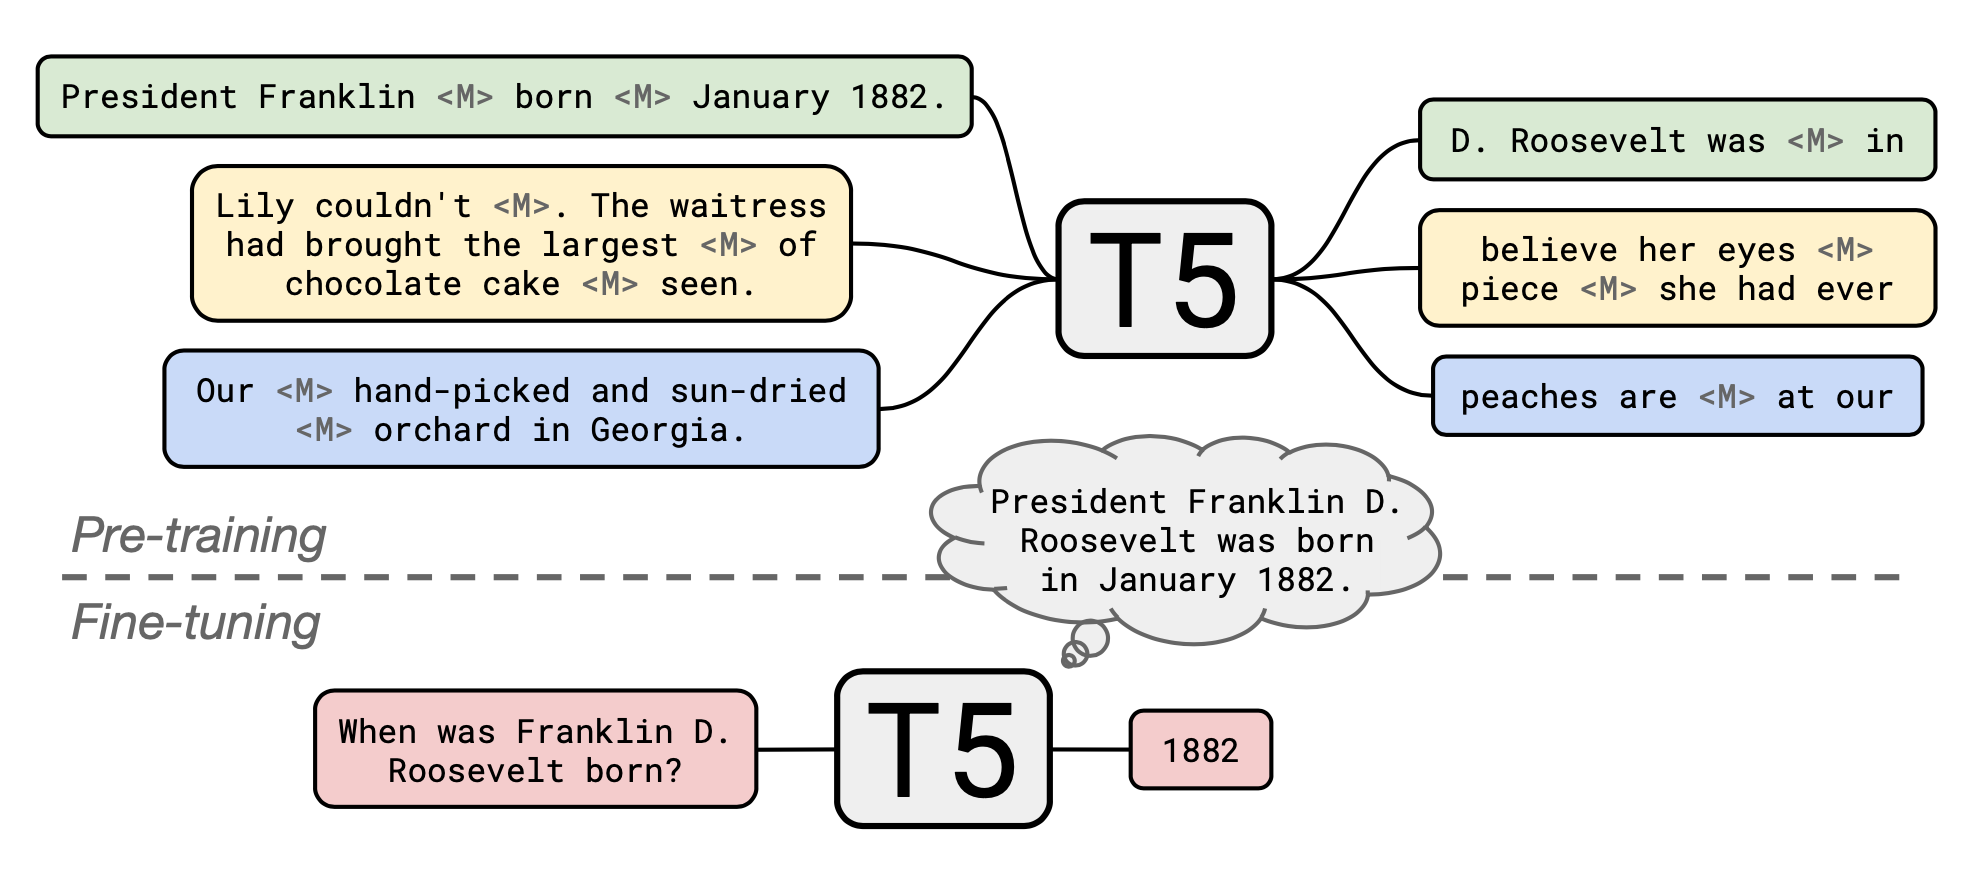
\includegraphics[width=\linewidth]{img/arch/T5_SSM.png}
    \caption{Mô hình T5 được fine-tuned để trả lời câu hỏi}
    \label{fig:arch_t5}
\end{figure}

Ngoài ra, trong một số trường hợp, một mô hình không nhất thiết cần phải được fine-tuned để có thể sử dụng trong việc trả lời câu hỏi, chẳng hạn như mô hình GPT-3. Theo đó, trong một bài báo được giới thiệu bởi \href{https://arxiv.org/abs/2005.14165}{Brown et al., 2020}, họ đã đánh giá khả năng trả lời câu hỏi của mô hình qua 3 trường hợp cụ thể như sau:

\begin{enumerate}
    \item \textbf{few-shot learning:} mô hình GPT-3 có thể nhận được một số chỉ dẫn về ngữ cảnh,
    \item \textbf{one-shot learning:} mô hình GPT-3 chỉ được nhận duy nhất \textbf{một} chỉ dẫn về ngữ cảnh,
    \item \textbf{zero-shot learning:} mô hình GPT-3 không được nhận bất kỳ một chỉ dẫn nào về ngữ cảnh.
\end{enumerate}

Theo đó, với tập dữ liệu TriviaQA, khả năng của mô hình GPT-3 có thể đạt được tương đương, hoặc thậm chí còn vượt trội hơn so với một mô hình khác đã được fine-tuned. Ngoài ra, cũng có thể thấy khả năng hoạt động của GPT-3 tỉ lệ thuận với kích cỡ của mô hình, như Hình \ref{fig:arch_gpt3} dưới đây.

\begin{figure}[h!]
    \centering
    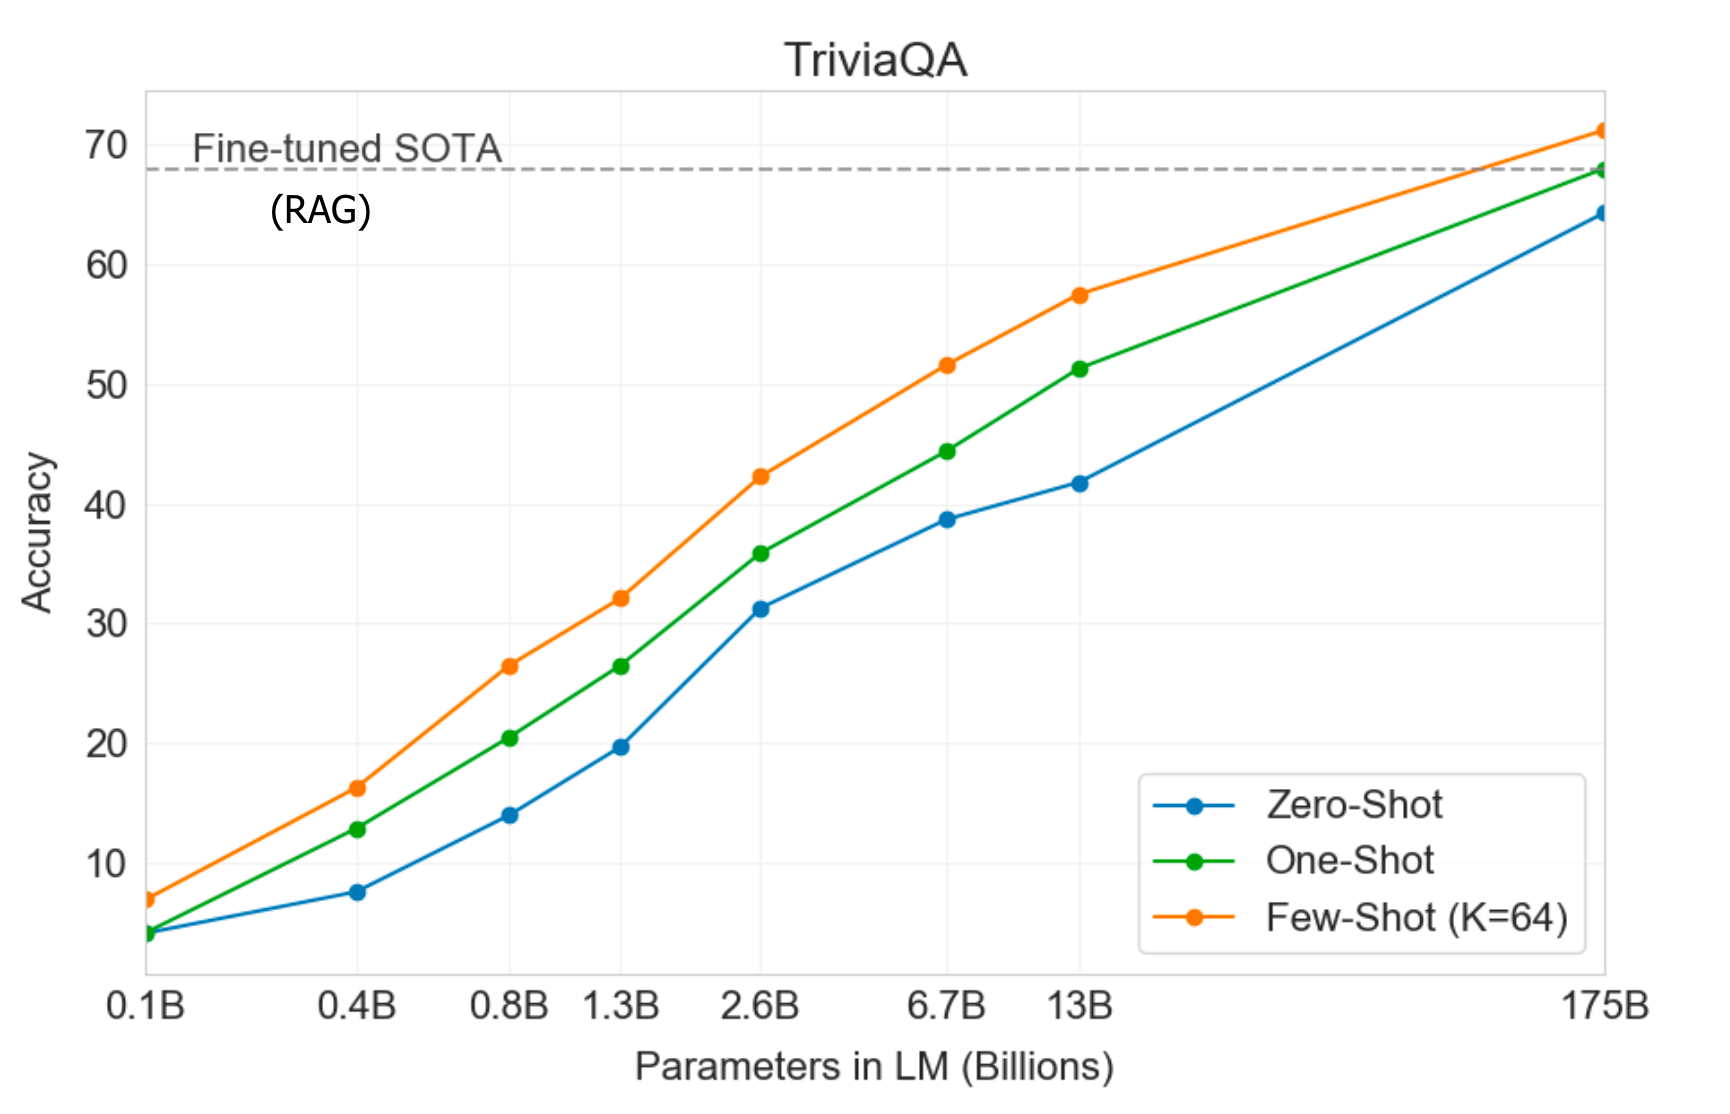
\includegraphics[width=\linewidth]{img/arch/GPT3-triviaqa.png}
    \caption{Khả năng của GPT-3 đối với tập dữ liệu TriviaQA}
    \label{fig:arch_gpt3}
\end{figure}